The study of nature at the quantum level has been at the forefront of physics since the early $20^{\textrm{th}}$ century. 
\dots

Here we will only introduce concepts utilised in this thesis.
For completeness, we elucidate some fundamental topics of linear algebra and quantum theory in \cref{apdx:fundamentals},
    but consider them too cumbersome to include in the main text. 
For a more complete and general introduction to \gls{qm}, the reader is referred to \cite{griffiths2018introduction, susskind2014quantum}.

\section{QM TODO}
\begin{easylist}[itemize]
    & Hamiltonian
    & Schrodinger equation
    & Unitary evolution

    & states
    && qubits
    & Hilbert space
    && pure/separable and mixed
    & operators/gates
    & Pauli matrices
    & Bloch sphere
    & measurement
    && projectors
    & expectation value
    & superposition/entanglement
    & first/second quantisation
    & quantum tech other than computation/simulation
\end{easylist}

\section{\glsentrylong{qm}}\label{sec:qm}

At any time, a quantum system, $Q$, can be described by its \emph{wavefunction}, $\Psi(t)$, 
    which contains all information about $Q$. 
In analogy with Newton's second law of motion, 
    which allows for the determination of a particle's position at any time, $\vec{r}(t)$, 
    given its conditions such as mass and acceleration as well as its initial position, $\vec{r}(t_0)$,  
    quantum \emph{equations of motion} can describe the evolution of $Q$ through its wavefunction \cite{dirac1981principles}. 
One proposal\footnotemark \ for the equation of motion 
    to describe the evolution of the wavefunction under known conditions, 
    i.e. determining $\Psi(t)$ from $\Psi(t_0) \ \forall t > t_0$, 
    is \emph{\schrodinger's equation}  \cite{griffiths2018introduction, mart2020introduce, nelson1966derivation}.
\footnotetext{
    The most noteworthy alternative formalism, due to Heisenberg \cite{heisenberg1985quantentheoretische}, 
    was shown equivalent to the \schrodinger picture described here.
}
\par 

Although the \schrodinger equation is a \emph{postulate} of \gls{qm} (see \cref{sec:postulates}), 
    let us introduce it in reverse order to elucidate its meaning, following \cite{susskind2014quantum}. 
We have yet to describe the structure of the wavefunction, which we will do in \cref{sec:quantum_info},
    but here we will represent wavefunctions using \emph{Dirac notation} (\cref{sec:dirac_notation}), 
    and can think of them generically as vectors, i.e. $\Psi(t) \rightarrow \ket{\psi(t)}$. 
Suppose we have two such wavefunctions, $\ket{\phi(t)}, \ket{\psi(t)}$ which are functions of time $t > t_0$.
We start with the assumption that \emph{similarity} is conserved between two wavefunctions,
    if they undergo the same transformation 
    (Susskind's \emph{minus first} law of classical mehcanics \cite{susskind2014quantum})
\begin{equation}
    \label{eqn:conservation_simularity}
    \braket{\phi(t) | \psi(t)} = \braket{\phi(t_0) | \psi(t_0)}
\end{equation}

Then, assuming some equations of motion capture the dynamics of $Q$, 
    there exists some evolution operator, $\hat{U}(t)$, which deterministically maps $\ket{\psi(t_o)}$ to $\ket{\psi(t)}$.
\begin{equation}
    \label{eqn:state_at_t}
    \ket{\psi(t)} = \hat{U}(t) \ket{\psi(t_0)},
\end{equation}
    where we have not yet imposed any restrictions on $\hat{U}$. 
Combining \crefrange{eqn:conservation_simularity}{eqn:state_at_t}, 
\begin{equation}
    \begin{split}
        \braket{\phi(t) | \psi(t)} &= \braket{ \phi(t_0) | \hat{U}^{\dag} \hat{U}| \psi(t_o) }
        \\
        \Rightarrow \braket{ \phi(t_0) | \hat{U}^{\dag}(t) \hat{U}(t) | \psi(t_o) } &= \braket{\phi(t_0) | \psi(t_0)}
        \\
        \Rightarrow \hat{U}^{\dag}(t) \hat{U}(t) &= \ident \ \ \ \ \forall t,
    \end{split}
\end{equation}
where the result $\hat{U}^{\dag}(t) \hat{U}(t) = \ident$ is the condition for \emph{unitarity} (\cref{sec:unitary}), 
    so we can claim the quantum wavefunction evolves unitarily. 
\par 

By construction, we require that after zero time, i.e. $t = t_0$, the wavefunction has not changed:
\begin{equation}
    \begin{split}
        \ket{\psi(t = t_0)} = \hat{U}(t = t_0)\ket{\psi(t_0)} = \ket{\psi(t_0)}
        \\ \Rightarrow \hat{U}(t = t_0) = \ident.
    \end{split}
\end{equation}
Without loss of generality we can set $t_0 = 0$, giving $\hat{H}(0) = \ident$. 
Then, let us consider an infintesimally small time increment $t_0 + \epsilon$:
    again, take $t_0 = 0$ so $t = \epsilon$,  where $\epsilon \gg \epsilon^2$. 

We can say
\begin{equation}
    \hat{U}(\epsilon) = \ident + \mathcal{O}(\epsilon),
\end{equation}
which merely suggests that the time evolution operator
    at very small time is very close to the identity, with some small displacement proportional to the time,
    which must be an operator to act on the wavefunction (vector).
We suppose the form of the offset, so we can write
\begin{equation}
    \hat{U}(\epsilon) = \ident - \epsilon \left(\frac{i}{\hbar} \ho \right),
\end{equation}
    where the inclusion of the phase $-i$ is arbitrary, 
    and we have named as $\nicefrac{\ho}{\hbar}$ the operator by which the time evolution differs from the identity. 
In other words, the operator $\ho$ is generically the generator of the evolution/dynamics of $Q$:
    any difference between $\ket{\psi(t_0)}$ and $\ket{\psi(t)}$ arises solely due to $\ho$. 
So far there is no restriction on $\ho$, 
    except that it must be of the same dimension as the Hilbert space in question. 
Recalling the unitarity condition, however:
\begin{equation}
    \label{eqn:hamiltonian_hermiticity}
    \begin{split}
        \hat{U}^{\dag}(\epsilon) \hat{U}(\epsilon) &= \ident
        \\ 
        \Rightarrow 
        \left( \ident + \frac{i}{\hbar} \epsilon \ho^\dag \right) \left( \ident - \frac{i}{\hbar} \epsilon \ho, \right)  &= \ident
        \\
        \Rightarrow
        \ident +  \frac{i}{\hbar} \epsilon (\ho^{\dag} - \ho) + \mathcal{O}(\epsilon^2) &= \ident
        \\
        \Rightarrow
        (\ho^{\dag} - \ho) = 0 
        \\
        \Rightarrow
        \ho^{\dag} = \ho.
    \end{split}
\end{equation}
\cref{eqn:hamiltonian_hermiticity} results in the condition for \emph{Hermiticity}, 
    meaning that $\ho$ is an observable of $Q$. 
In fact, this is the \emph{Hamiltonian} of the system, described in the next section. 

\par 
We can also use the infintesimal evolution to see 
\begin{equation}
    \label{eqn:derivation_schrodinger_eqn}
    \begin{split}
        \ket{\psi(t)} &= \hat{U}(t) \ket{\psi(t_0)}
        \\ \Rightarrow \ket{\psi(\epsilon)} &= \hat{U}(\epsilon) \ket{\psi(t_0)}
        \\ \Rightarrow 
        \ket{\psi(\epsilon)} &= \left(\ident - \epsilon \frac{i}{\hbar} \ho \right) \ket{\psi(t_0)}
        \\ \Rightarrow \ket{\psi(\epsilon)} &= \ket{\psi(t_0)} - \epsilon \frac{i}{\hbar} \ho \ket{\psi(t_0)}
        \\ \Rightarrow \frac{\ket{\psi(\epsilon)} - \ket{\psi(t_0)} }{\epsilon}  &= - \frac{i}{\hbar} \ho \ket{\psi(t_0)}
    \end{split}
\end{equation}
Taking the limit as $\epsilon \rightarrow 0 $, the left hand side of the final line of \cref{eqn:derivation_schrodinger_eqn} is the definition
    of the derivative of the wavefunction, $\frac{d \ket{\psi(t)}}{dt}$. 
Taken together, we have 
\begin{equation}
    \label{eqn:schrodinger}
    \frac{d}{dt} \ket{\psi(t)} = \frac{-i}{\hbar} \ho \ket{\psi(t_0)},
\end{equation}
    where $\ket{\psi(t)}$ is the wavefunction at time $t$, 
    $\ket{\psi(t_0)}$ is the wavefunction at $t_0$, such that $t > t_0$, 
    $\hbar = 1.054 \times 10^{-34}$ is the reduced Planck constant and 
    $\ho$ is the \emph{Hamiltonian} of $Q$. 
For brevity we generally refer to $t_0 = 0$, and absorb $\hbar$ into $\ho$, which will later manifest in the Hamiltonian scalar parameters. 
\cref{eqn:schrodinger} is the most general form of \emph{\schrodinger equation}, 
    otherwise known as the \emph{time-dependent} \schrodinger equation; 
    we include it as \Cref{postulate:schrodinger_eqn} when describing the fundamentals of \gls{qm} (\cref{sec:postulates}), 
    since it can be seen as an irreducible equation of motion which is essential to the description of quantum systems. 

\par 


\subsection{Hamiltonians}\label{sec:hamiltonians}
In the previous section we introduced the Hamiltonian\footnotemark \ of $Q$ as the generator of its 
    time evolution dynamics;
    Hamiltonians are of primary importance in this thesis, so it is worth pausing to consider their physical meaning. 
We saw in \cref{eqn:hamiltonian_hermiticity} that $\ho$ is Hermitian, 
    meaning that the operator is physically observable 
    according to \Crefrange{postulate:eigenvalues}{postulate:hermiticity}
    of \glsentrylong{qm} (\cref{sec:postulates}). 
The Hamiltonian operator captures the energy of $Q$: 
    the eigenvalues of the observable $\ho$ are the permitted energy levels of the system.
\par 

The quantum Hamiltonian, $\ho$ is analogous to the classical Hamiltonian, 
    insofar as it captures all the interactions of a given system which contribute to its time evolution.
Knowing the classical Hamiltonian and the initial conditions -- position and momentum -- 
    Hamilton's equations of motion allow for the calcaultion of those quantities for the particle 
    in question an infintesimal time later \cite{susskind2014classical}.    
Likewise, knowledge of the initial wavefunction, $\ket{\psi(t_0)}$, and the system's quantum Hamiltonian, $\ho$, 
    the quantum equations of motion -- \schrodinger's equation, \cref{eqn:schrodinger} -- 
    permits the calculation of the wavefunction at later times.
As such the Hamiltonian must consist of all processes which influence the evolution of $Q$;
    we will later break the Hamiltonian into independent \emph{terms} which each correspond to unique physical interactions
    $Q$ is subject to, \cref{sec:models}. 
We can think that each process/interaction $Q$ undergoes contributes to its total energy,
    giving intuition as to why its eigenvalues are the energy levels. 
\par 
\footnotetext{
    Aside: the author shares a hometown with the mathematician for whom it is named, William Rowan Hamilton. 
    It is hoped that, after another 150 years, the next physicist from Trim, Co. Meath, Ireland might 
    profitably use knowledge Hamiltonians on a quantum computer. 
}

Hamiltonians describe \emph{closed} quantum systems, 
    i.e. where \emph{all} processes and interactions which influence $Q$ are accounted for. 
Realistic quantum systems are influenced by a myriad of proximal systems, 
    and it is therefore infeasible to analytically account for them all. 
Instead, \emph{open} quantum systems' dynamics are described by Lindbladian operators, which encompass the Hamiltonian form. 
The Lindblad master equation is a generalisation of the \schrodinger equation, 
    providing the equation of motion for open quantum systems \cite{breuer2002theory, manzano2020short}.
In this thesis we only consider closed models for quantum systems;
    for meaningful impact of the techniques presented here, it will be necessary to expand them to account for the open system dynamics of realistic experiments.
We do, however, show initial progress towards this endeavour by modelling a physical system through a closed Hamiltonian, \cref{chapter:nv}.
\par 

%%%%%%%%%%%%% QUANTUM INFORMATION %%%%%%%%%%%%%
\section{Quantum Information}\label{sec:quantum_info}
We have not yet described the structure of the wavefunction, 
    instead performing the previous analysis with respect to some arbitrary objects.
The wavefunction for a physical system, $Q$, is also known as its \emph{state}, 
    a complete mathematical description of the system \cite{preskill1998lecture}.
States are vectors\footnotemark, $\ket{\psi} \in \mathbb{C}$;
    the valid state space for $Q$ is its \emph{Hilbert space}, $\hilbert$,
    which is a generalisation of Euclidean vector space, 
    i.e. $\ket{\psi} \in \hilbert$. 
\footnotetext{We immediately use Dirac notation to represent the state; it is defined in \cref{sec:dirac_notation}.}
The Hilbert space defines the overlap between any two vectors as the \emph{inner product}, $\braket{\psi | \phi}$ (\cref{sec:linear_algebra}). 
In general\footnotemark, a state can be seen as a \emph{superposition} across its eigenstates, $\left\{\ket{i}\right\}$.  
\footnotetext{We expand on this brief description in \cref{sec:states}.}

\begin{subequations}
    \begin{equation}\label{eqn:state_vector}
        \ket{\psi} = \sum\limits_{i} \alpha_i \ket{i}
    \end{equation}
    \begin{equation}\label{vector_norm}
        \textrm{subject to} \ \ \ \sum\limits_{i} |\alpha_i|^2 =1, \ \ \ \alpha_i \in \mathbb{C}. 
    \end{equation}
\end{subequations}

The cornerstone of \gls{qm} is the effect of \emph{measurement} on quantum systems: 
    in general $Q$ can be seen as occupying a multitude of eigenstates as in \cref{eqn:state_vector}, 
    observing the system forces $\ket{\psi}$ into a definite occupation of a single eigenstate,
    where the \emph{probability} that it is measured in each eigenstate $\ket{i}$ is given by $\absval{\alpha_i}^2$, 
    according to Born's rule \cite{born1926quantenmechanik}.
$\alpha_i$ are hence named \emph{probability amplitudes} since they inform the probability of measuring the corresponding eigenstate. 
\par 

For an ideal\footnotemark \ single particle, when the state, \cref{eqn:state_vector}, has two available eigenstates, 
    e.g. the horizontal ($H$) and vertical ($V$) polarisation of a single photon, 
    we can designate $Q$ as a two-level computational platform, called a \emph{qubit}, 
    analogous to the workhorse of classical computation, the bit. 
A qubit's state vector can then be written as a sum over the two available eigenstates, 
    where we assign vectors to the eigenstates as $\left{ \ket{H} = \ket{v_1}, \ket{V} = \ket{v_2}$. 
\footnotetext{
    Here we restrict to the space of ideal, \emph{logical} qubits. In reality, physical qubits are beset by errors, 
    demanding error correction routines such that multiple particles are needed attain a single logical qubit. 
}
\begin{equation}
    \label{eqn:qubit_state}
    \ket{\psi} = \alpha_1 \ket{v_1} + \alpha_2 \ket{v_c},
\end{equation}
where $\alpha_i \in \mathbb{C}$ and $\absval{\alpha_1}^2 + \absval{\alpha_2}^2 = 1$. 
\par

In general, a qubit requires two orthogonal state vectors to define a \emph{basis};
    we list a number of the usual special cases:
\begin{subequations}
    \label{eqn:bases}
    \begin{equation}
        \label{eqn:basis_x}
        X\textrm{-basis} = \left\lbrace \begin{split}
        \ket{+} &= \frac{1}{\sqrt{2}} \left( \ket{0} + \ket{1} \right)
        \\
        \ket{-} &= \frac{1}{\sqrt{2}} \left( \ket{0} - \ket{1} \right)
        \end{split}
        \right.
    \end{equation}
    \begin{equation}
        \label{eqn:basis_y}
        \begin{split}
        Y\textrm{-basis} = \left\lbrace 
        \begin{split}
            \ket{i} &= \frac{1}{\sqrt{2}} \left( \ket{0} + i \ket{1} \right)
            \\
            \ket{-i} &= \frac{1}{\sqrt{2}} \left( \ket{0} - i \ket{1} \right)
        \end{split}
        \right.        
        \end{split}
    \end{equation}
    \begin{equation}
        \label{eqn:basis_z}
        Z\textrm{-basis} = \left\lbrace \begin{split}
            &\ket{0}
            \\
            &\ket{1}
            \end{split}
            \right.
    \end{equation}
\end{subequations}

A visual tool for representing qubits is the \emph{Bloch sphere}, 
    which presents orthogonal basis states as parallel unit vectors of opposite direction:
    we show each of the bases of \cref{eqn:bases} in \cref{fig:bases}. 

\begin{figure}
    \begin{center}
        \subfloat{
            % 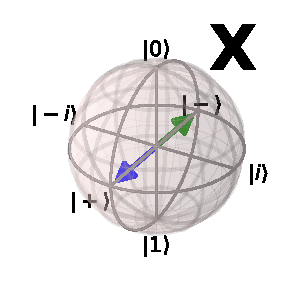
\includegraphics[width=0.3\textwidth]{contextual_review/figures/bloch_x_axis.pdf}
            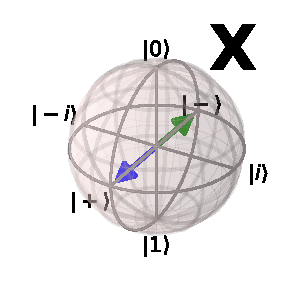
\includegraphics{contextual_review/figures/bloch_x_axis.pdf}
        }
        \qquad
        \subfloat{
            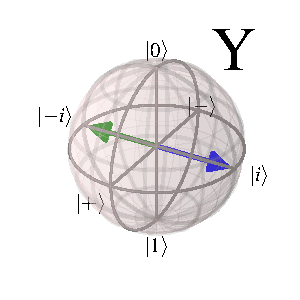
\includegraphics{contextual_review/figures/bloch_y_axis.pdf}
        }
        \qquad
        \subfloat{
            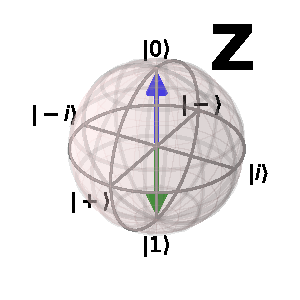
\includegraphics{contextual_review/figures/bloch_z_axis.pdf}
        }
        \qquad
    \end{center}
    \caption[Bloch sphere representation of bases]{
        Bloch sphere representation of bases, where each pair of basis states are shown by blue and green vectors. 
        The $X$-basis has basis vectors $\left\{ \ket{+}, \ket{-}\right\}$; $Y$-basis has $\left\{ \ket{i}, \ket{-i}\right\}$ 
            and $Z$-basis has $\left\{ \ket{0}, \ket{1}\right\}$.
    }
    \label{fig:bases}
\end{figure}

We can make two remarks about basis states for a single qubit:
\begin{easylist}[itemize]
    & Basis states from one basis can be seen as superpositions with respect to alternative bases
    && e.g. in the $X$-basis, $\ket{+}$ is a basis vector, but in the $Z$-basis, $\ket{+} = \frac{\ket{0} + \ket{1}}{\sqrt{2}}$ is a superposition over basis vectors. 
    & Bases are local rotations of each other
    && rotating the $X$-basis through an angle $\nicefrac{\pi}{2}$ about the $Y$-axis results in the $Z$-axis.
\end{easylist}

\par 

As we alluded to in \cref{sec:qm}:
    by imposing mathematical structure on quantum systems' states, 
    i.e. representing $Q$ as a state vector at any time, 
    then operations which alter the state of the system must be matrices. 
In general an $n$-dimensional vector is rotated by an $n \times n$ matrix;
    here one-qubit oeprators have the effect of rotating the state vector, 
    which we can again visualise on the Bloch sphere.
By thinking of qubits generically with respect to any basis, we can encode information in the qubit's amplitudes,
    by performing operations (or \emhp{gates}) upon the qubit, we change the information, 
    i.e. we can design information processing techniques leveraging the infrastructure -- states, operators and measurement -- of \gls{qm}. 
\par 

We introduce a set of speical one-qubit operators, the \emph{Pauli matrices},  

\begin{subequations}
    \begin{equation}
        \sx = \begin{pmatrix}
            0 & 1 \\
            1 & 0 
        \end{pmatrix}
    \end{equation}        
    \begin{equation}
        \sy = \begin{pmatrix}
            0 & -i \\
            i & 0 
        \end{pmatrix}
    \end{equation}        
    \begin{equation}
        \sz = \begin{pmatrix}
            1 & 0 \\
            0 & -1 
        \end{pmatrix}
    \end{equation}        
\end{subequations}

The Pauli matrices are used to define rotation operators about 
    their respective axes, and hence are very useful:
    we can break \emph{any} rotation of a qubit into rotations of various angles, $\theta$, about the three axes of the Bloch sphere.
Any single qubit operation can therefore be expressed as a product of
    the \emph{rotation operators}, $\hat{R}_x, \hat{R}_y, \hat{R}_z$, exemplified in \cref{fig:bloch_rotations} and defined as
\begin{equation}
    \label{eqn:rotation_operator}
    \begin{split}
        \hat{R}_w\left(\theta) &= e^{i \frac{\theta}{2} \hat{\sigma}_w} 
        = \cos\left(\nicefrac{\theta}{2}\right) \ident + i \sin \left(\nicefrac{\theta}{2}\right) \hat{\sigma}_w.
    \end{split}
\end{equation}
    
\par
The Pauli matrices are Hermitian, meaning they are observable. 
We can see that the eigenstates of $\sz$ are the $Z$-basis states:
    $\sz \ket{0} = \ket{0}; \sz \ket{1} = - \ket{1}$.
Recalling the earlier claim that the two-level quantum system (e.g. $H$ and $V$ polarisation of a photon)
    can be mapped to eigenvectors\footnotemark of an obserable operator to form a qubit, 
    we term the $Z$-basis the \emph{computational} basis.
By defining the computational basis, we ground abstract computational reasoning in the physical realisation:
    anywhere throughout this thesis where the basis states $\ket{0}, \ket{1}$ are referenced, 
    we mean the eigenstates of the physical axis which is defined as the $Z$-axis for the system in question. 
\footnotetext{
    The terms \emph{eigenstate} and \emph{eigenvector} are interchangeable, 
    although it may be helpful to think of eigenstate as the physical manifestation (horizontal photon), 
    and think of eigenvector as the logical manifestions ($\ket{0}$). 
}
In the computational basis, then, a qubit can be specified as
\begin{equation}
    \label{eqn:computational_qubit}
    \ket{\psi} = \alpha_0 \ket{0} + \alpha_1 \ket{1}.
\end{equation}

\begin{figure}
    \begin{center}
        \subfloat{
            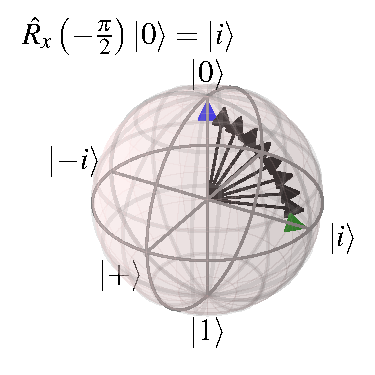
\includegraphics{contextual_review/figures/bloch_rotate_x.pdf}
        }
        \qquad
        \subfloat{
            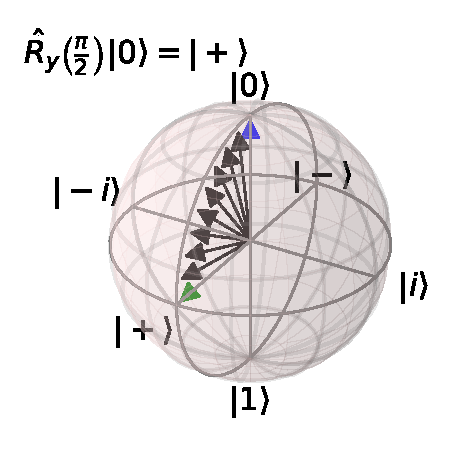
\includegraphics{contextual_review/figures/bloch_rotate_y.pdf}
        }
    \end{center}
    \caption[Rotations on Bloch sphere]{
        Rotations on Bloch sphere. 
        The initial and final state are shown in blue and green respectively, while intermediate states are shown in black. 
        \textbf{Left}, The $Z$-basis unit vector, $\ket{0}$, is rotated about the $X$-axis, resulting in the unit vector along the $Y$-axis. 
        \textbf{Right}, The $Z$-basis unit vector, $\ket{0}$, is rotated about the $Y$-axis, resulting in the unit vector along the $X$-axis. 
    }
    \label{fig:bloch_rotations}
\end{figure}
    

\subsection{Multipartite systems}
Qubits can then be interfaced together, where the resultant states are spanned by the Pauli group
\par 

\subsection{Expectation value}
The projection operator projects the state onto eigenstates. 

We can get the expectation value.. 
Especially for this thesis, there is a subtlety to be aware of: 
    in later chapters, we will make reference to the expectation value and likelihood, 
    almost interchangeably -- these are distinct concepts that \emph{sometimes} overlap, but not in all cases. 
Moreover, the likelihood usually refers 


\section{Quantum Computation and Simulation}
\begin{easylist}[itemize]
    & Algorithms
    && advantage
    & Hardware
\end{easylist}

Supremacy proposals: \cite{harrow2017quantum}
\par 

Bringing together the concepts of the chapter so far, 
    we can use qubits to represent the state of real quantum systems. 
This allows for efficient simuation of processes at the quantum level for the first time, 
    facilitiating novel insights of nature's most intricate details. 

